\documentclass{article}
\usepackage{geometry}
\usepackage{graphicx}
\usepackage{subcaption}
\usepackage{placeins}
\usepackage{hyperref}
\usepackage{url}

\title{BME 599: Advanced Topics in MRI\\HW \#2}
\author{Tom Griesler}

\geometry{left=2cm, right=2cm, top=1cm}

\date{\today}
\begin{document}

\maketitle

\section{Problem 1: Extended phase graphs}
\textbf{Shown below is a sequence diagram of a fast spin echo (FSE) with its first 8 refocusing pulses within one repetition time (TR). Each RF pulse is designated as a delta function, so you do not need worry about the slice profile. Refocusing pulses are spaced 5ms apart (echo spacing).}

\begin{itemize}

    \item[a.] Please write a function using EPG to simulate spin echo train echo amplitudes for a sequence with $90$°$_x$ excitation, followed by refocusing pulses of $[\alpha+(90- \alpha/2)]_y$ , $\alpha_y$, $\alpha_y$ ,... for 64 echoes for $T1 = [200:100:1500]\,$ms, and $T2 = [50:30:300]\,$ms
    
        \begin{itemize}

            \item[i.] Simulate echo amplitudes with $\alpha = 180$°, and plot amplitudes with five different T1 and T2 combinations
            
                \begin{figure}[h!]
                    \centering
                    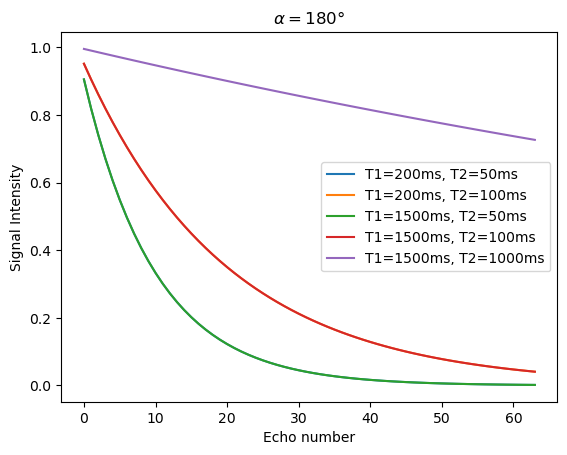
\includegraphics[width=0.5\textwidth]{figures/1_a_i.png}
                    \caption{}
                    \label{}
                \end{figure}

            \item[ii.] Simulate echo amplitudes with $\alpha = 120$°, and plot amplitudes with five different T1 and T2 combinations
            
                \begin{figure}[h!]
                    \centering
                    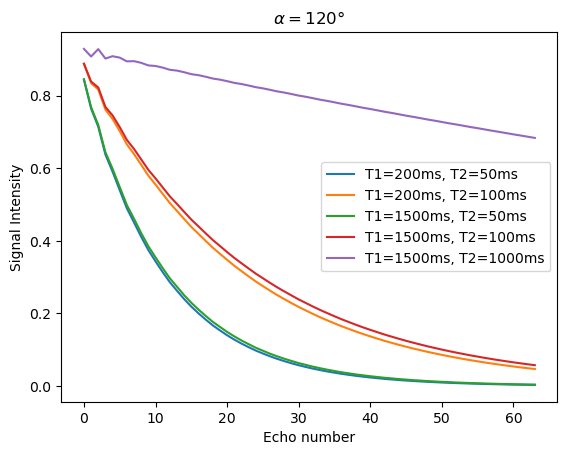
\includegraphics[width=0.5\textwidth]{figures/1_a_ii.png}
                    \caption{}
                    \label{}
                \end{figure}
            
            \item[iii.] Simulate echo amplitudes with $\alpha = 60$°, and plot amplitudes with five different T1 and T2 combinations
            
                \begin{figure}[h!]
                    \centering
                    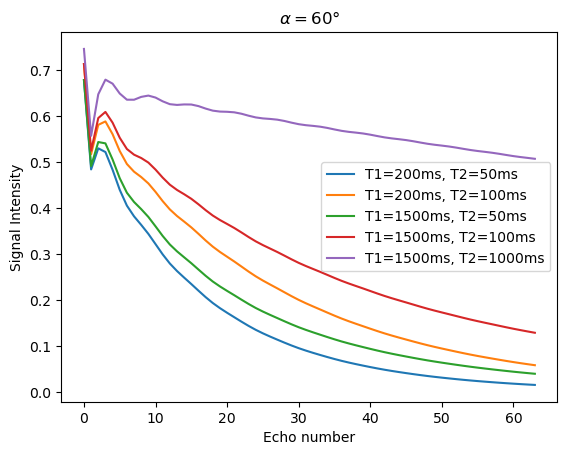
\includegraphics[width=0.5\textwidth]{figures/1_a_iii.png}
                    \caption{}
                    \label{}
                \end{figure}

        \end{itemize}

\end{itemize}

\end{document}